In this Section we describe how we've stumbled upon an incredible manifestation of perimeter and $\gamma$ constancy, involving simple measures in a triangle, and its surprising corollaries.

Denote the radii of an $N=3$ orbit's Incircle, Circumcircle, and 9-Point Circle \cite{mw} as $r$ (Inradius) $R$ (Circumradius) and $r_9$, respectively,  Figure~\ref{fig:radii}.

\begin{figure}[H]
    \centering
    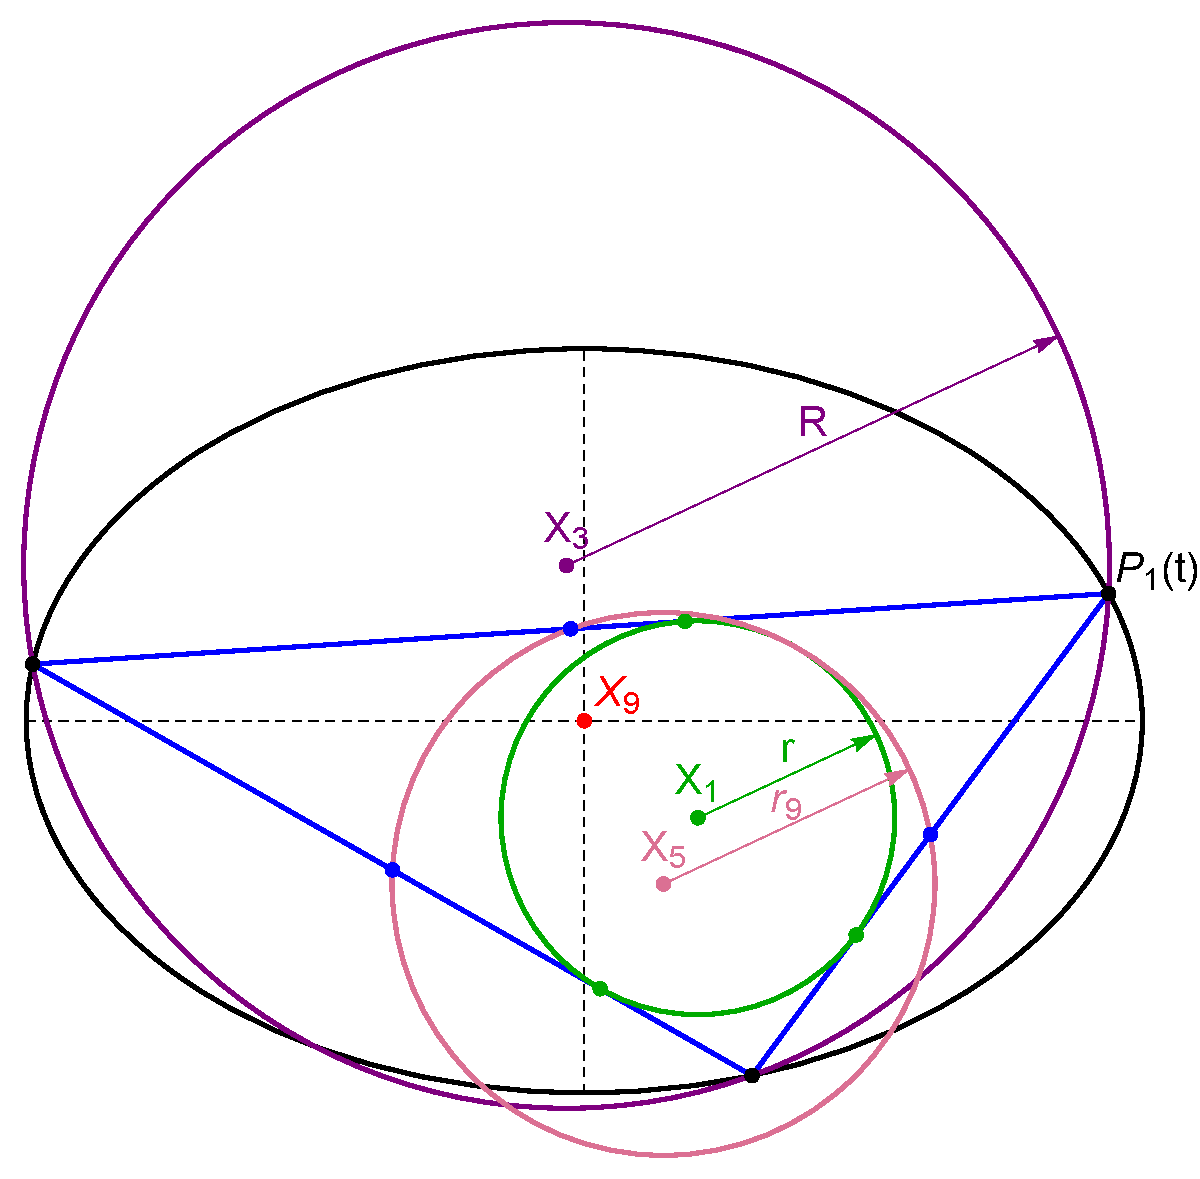
\includegraphics[width=.65\textwidth]{pics/u0070_Radii.pdf}
    \caption{A 3-periodic (blue), a starting vertex $P_1$, the Incircle (green), Circumcircle (purple), and 9-Point Circle (pink), whose centers are $X_1$, $X_3$, and $X_5$, and radii are the inradius $r$, circumradius $R$, and 9-Point Circle radius $r_9$.}
    \label{fig:radii}
\end{figure}

\noindent The relation $R/r_9=2$ is well-known \cite{mw}. Remarkably \cite{ronaldo19a}:

\begin{theorem}
A 3-periodic family conserves the $r/R$ ratio. 
\label{thm:rovR}
\end{theorem}

Specifically, $r/R$ can be expressed in terms of two known constants of motion: perimeter and angular momentum \cite{dominique19,sergei19_private_circles}, as follows:

\begin{equation}
\frac{r}{R}=%\frac{2(\delta-1)}{(a^2-1)(\delta+a^2)}=
\gamma L - 4\, .
\label{eqn:rR_dominique}
\end{equation}

Additionally, it can be shown that when the EB is circular, $r/R$ is maximal at $0.5$ (orbits are equilaterals). As $a/b\rightarrow\infty$, the ratio goes to zero.

\subsection{Conservation of the Sum of Cosines}

Denote $\theta_i,i=1,2,3$ the angles internal to the orbit. The following is an identity valid for any triangle \cite{johnson29}:
%
\begin{equation}
\sum_{i=1}^{3}{\cos\theta_i}=1+\frac{r}{R}\;.
\label{eqn:rR_cos}
\end{equation}

Since the right-hand side is constant, so must be the sum of the cosines! So a corollary to Theorem~\ref{thm:rovR} is:

\begin{corollary}
\label{cor8}
A 3-periodic family conserves the sum of cosines. 
\end{corollary}

\subsection{Conservation of the Product of Excentral Cosines}

A triangle is always the Orthic of its Excentral \cite{mw}. If $\theta_i'$ are the Excentral's angles, the following is a known relation \cite{johnson29}:

\begin{equation}
\prod_{i=1}^{3}{|\cos\theta_i'|}=\frac{r}{4R}\;.
\label{eqn:prod-cos}
\end{equation}

Let $\theta_i'$ be an angle of the Excentral Triangle opposite to orbit angle $\theta_i$. It can be shown that $\theta_i'=\frac{\pi-\theta_i}{2}$, i.e., the Excentral Triangle is acute. Therefore the absolute sign in Equation~\ref{eqn:prod-cos} can be dropped. Since the right hand side of the above is constant:

\begin{corollary}
\label{cor9}
A 3-periodic family conserves the product of Excentral cosines. 
\end{corollary}

\begin{figure}
    \centering
    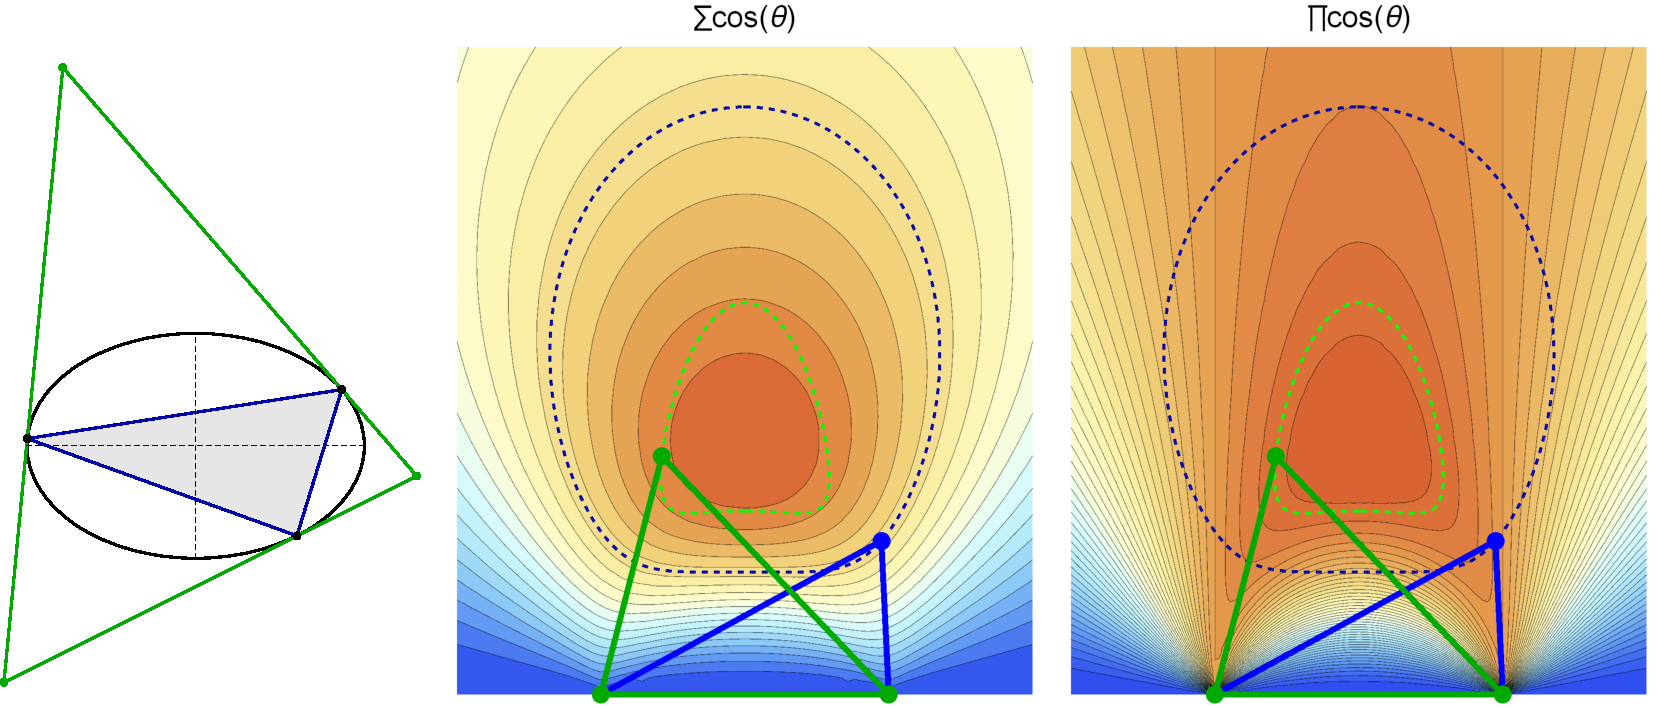
\includegraphics[width=\textwidth]{pics/u0072_cosine_conservation_small.pdf}
    \caption{\textbf{Left}: the EB (black), an $N=3$ orbit (blue), and its Excentral Triangle (green). \textbf{Middle}: both the orbit and its Excentral are shown in an ``elementary'' configuration: two vertices are pinned to the $x$ axis and a third one is set free, in such a way that triangles here are similar to their counterparts on the left. Isocurves of constant cosine sum are shown in terms of the position of the free vertex. Notice only the orbit triangle follows such an isocurve (dashed blue). \textbf{Right}: Here isocurves of cosine product are shown, showing the free vertex of the Excentral Triangle moves along one (dashed green).  \href{https://youtu.be/P8ykpE_ZbZ8}{Video}  \cite[pl\#15]{dsr_math_intell_playlist}}
    \label{fig:conserve_cosines}
\end{figure}

\noindent Figure~\ref{fig:conserve_cosines} illustrates conservation of sum (resp. product) of $N=3$ orbit (resp. Excentral Triangle) cosines.

\subsection{Conservation of Excentral-to-Orbit Area Ratio}

Let $A$ be the area of some triangle and $A_h$ the area of its Orthic. A well-known relation is that the ratio $A/A_h$ is inversely proportional to the Inradius-to-Circumradius ratio of the Orthic \cite{johnson29}:

\begin{equation}\label{eqn:AAh}
\frac{A}{A_h}=\frac{2R_h}{r_h}\;. 
\end{equation}

\noindent Since the orbit is its Excentral's Orthic, $r/R$ constant implies:

\begin{corollary}
\label{cor10}
A 3-periodic family conserves the Excentral-to-Orbit area ratio.
\end{corollary}
